\subsection{Information System Description}
Figure \ref{System overview} gives an overview of the system components for sourcing, extracting, enriching and integrating the  data and making the resulting structured and higher level information available to the user's analysis.

\begin{figure}[h]
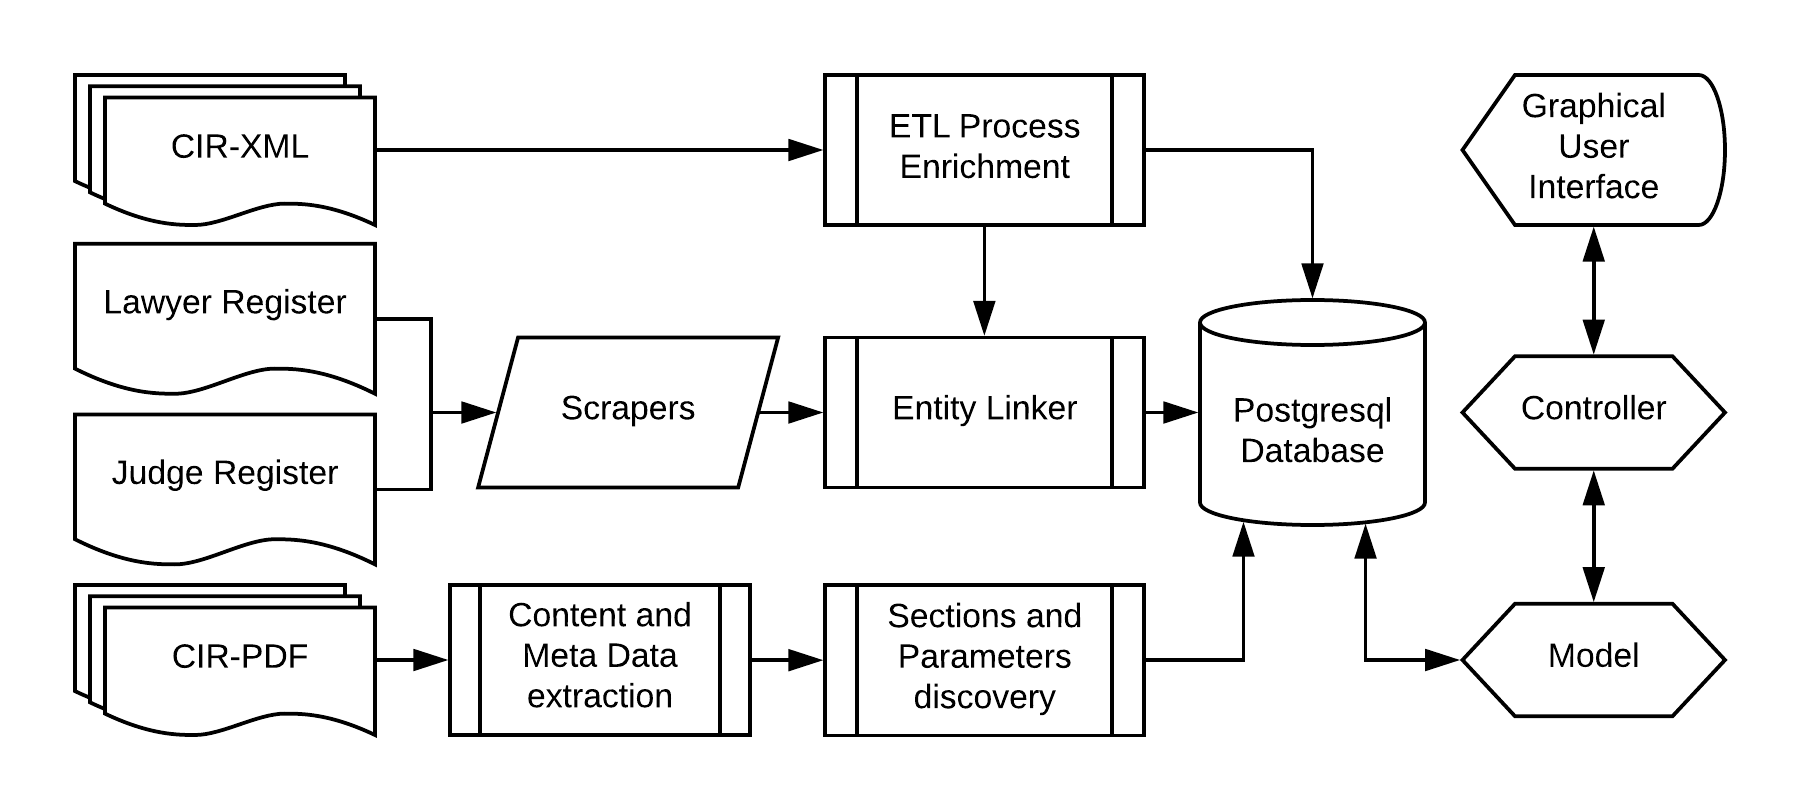
\includegraphics[width=1\linewidth]{images/system_overview.png}
\caption{System overview.}\label{System overview}
\end{figure}

Data flows from left to right through the following components:

\paragraph{Data Sources} Data is sourced from three public registers:
\begin{enumerate}
	\item The Central Insolvency Register (\textit{Centraal Insolventie Register or CIR}). CIR exposed both an XML and PDF file web service.
	\item The Register of lawyers (\textit{NOvA's Tableau}).
	\item The Register of ancillary positions of judges. (\textit{Register van nevenfuncties van rechters}) 
\end{enumerate}

The CIR provides the bulk of the data. The other two registers are used for the entity resolution of administrators and judges.

\paragraph{ETL and Enrichment} This component loads entities with selected data fields from the CIR XML data. The data is cleaned and enriched after which it is stored in a relational database.

\paragraph{Entity Linker} This component is responsible for linking judges and administrators in the CIR XML data to real life entities found in the judge and lawyer registers. 

\paragraph{PDF Processors}
These components processes the CIR PDF reports to extract textual content and meta data. The text sections as defined in the progress report template and key data parameter are discovered in a subsequent process and loaded into the relational database.

\paragraph{Database and File Storage}
Entity data is stored in a relational Postgresql database. Administrator PDF reports are stored in Amazon's S3 object storage.

\paragraph{Model-View-Controller (MVC)}
This well established pattern of subcomponents works together as a graphical interface for the user to analyse the data. 
%The user operates a graphical interface, prototyped in Jupyter notebooks, to query the data or interact with data visualisations or tables. The interface is the View in the MVC component. On user command, the Controller asks the Model to prepare the necessary data and then passes this data to the View to update the interface.
